
\section{Omitted Proofs}
\label{sec:omitted}

\begin{proof}[Proof of Theorem~\ref{thm:improve}]
Define the weight function $w'(e)
= \floor{\frac{w(e)}{w_{\max}} \cdot \frac{m}{2\eps}}$, where
$w_{\max} \eqdf \max_{e \in A} w(v)$.
%
Let $M^*$ and $M'$ be an optimal carpool matchings with respect to $w$
and $w'$, resp.  We have that
\[
w'(M^*)
=    \sum_{e \in M^*} \floor{\frac{w(e)}{w_{\max}} \cdot \frac{m}{2\eps}}
>    \sum_{e \in M^*} \paren{ \frac{w(e)}{w_{\max}} \cdot \frac{m}{2\eps} } - m
=    \frac{m}{2\eps w_{\max}} \cdot w(M^*) - m
~.
\]
Since $w(M^*) \geq w_{\max}$, we have that 
\[
w'(M^*)
>    \frac{m}{2\eps w_{\max}} \cdot (w(M^*) - 2\eps w_{\max})
\geq \frac{m}{2\eps w_{\max}} \cdot (1 - 2\eps) w(M^*)
~.
\]
By Theorem~\ref{thm:improve-bounded}, our local improvement algorithm computes a
$\half$-approximate carpool matching $M$ on $(G, c, w')$, and this
matching satisfies $w'(M) \geq w'(M')/2$.  Furthermore, since
$w'(M') \geq w'(M^*)$, it follows that $w'(M) \geq w'(M^*)/2$.
Therefore
\[
w(M)
\geq \frac{2\eps w_{\max}}{m} w'(M) 
\geq \frac{1}{2} \frac{2\eps w_{\max}}{m} w'(M^*)
>    \frac{1-2\eps}{2} w(M^*)
~,
\]
as required.
\end{proof}

\medskip

\begin{proof}[Proof of Lemma~\ref{lemma:dec}]
We give a constructive proof.
%
First, if $\ell \leq |V| \leq \Delta \ell$, then we are done.
%
Otherwise, we partition the graph recursively as follows.  Let $U
= \emptyset$.  As long as $\abs{U} < \ell$, choose an arbitrary vertex
$u$ such that $U \cup \set{u}$ is connected and add $u$ to $U$.
%
If the graph $G[V \setminus U]$, which is induced by $V \setminus U$,
is connected, then choose the next vertex.
%
However, if $G[V \setminus U]$ becomes disconnected, then consider the
maximal connected components of $G[V \setminus U]$.  Add the vertices
of any maximal component that contains less than $\ell$ vertices to
$U$.  Observe that afterwards $\abs{U} < \ell + (\Delta-1) \ell
= \Delta \ell$.
%
If $\abs{U} \geq \ell$, then recursively partition any component of
$G[V \setminus U]$ that contains more than $\ell$ vertices.
%
If $\abs{U} < \ell$, then there must exist at least one maximal
component $C$ of $G[V \setminus U]$ that contains more than $\ell$
vertices.  In this case recursively partition any maximal component of
$G[V \setminus (U \cup C)]$ that contains more than $\ell$ vertices.
Also, continue to augment $U$ in the graph $G[U \cup C]$.
\end{proof}


%%%%%%%%%%%%%%%%%%%%%%%%%%%%%%%%%

\newpage

\section{Figures}
%\label{sec:figures}

\begin{figure}[h]
\centering
\begin{subfigure}{.45\linewidth}
\centering
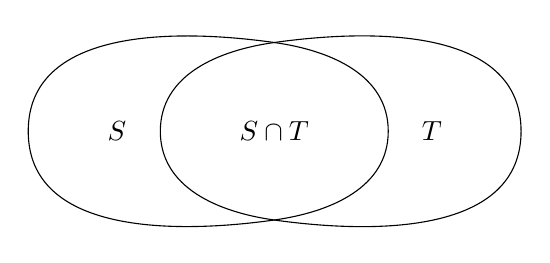
\begin{tikzpicture}[]

\begin{scope}[every node/.style={inner sep=1cm}]
\node(s) at(-2,0) {$S$};
\node(st) at(0,0) {$S \cap T$};
\node(t) at(2,0) {$T$};
\end{scope}

\draw 
(s.west) to[out=90, in=172] 
(st.north) to[out=-8, in=90] 
(st.east) to[out=270, in=8]
(st.south) to[out=188, in=270]
(s.west)
;

\draw 
(t.east) to[out=90, in=8] 
(st.north) to[out=188, in=90] 
(st.west) to[out=270, in=172]
(st.south) to[out=-8, in=270]
(t.east)
;

\end{tikzpicture}
\end{subfigure}
%
\hfill
%
\begin{subfigure}{.45\linewidth}
\centering
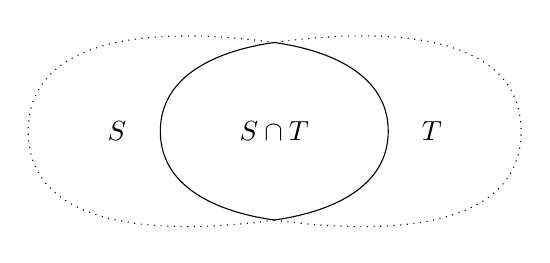
\begin{tikzpicture}[]

\begin{scope}[every node/.style={inner sep=1cm}]
\node(s) at(-2,0) {$S$};
\node(st) at(0,0) {$S \cap T$};
\node(t) at(2,0) {$T$};
\end{scope}

\draw[dotted] 
(st.south) to[out=188, in=270]
(s.west) to[out=90, in=172] 
(st.north)
;
\draw 
(st.north) to[out=-8, in=90] 
(st.east) to[out=270, in=8]
(st.south)
;

\draw[dotted] 
(st.south) to[out=-8, in=270]
(t.east) to[out=90, in=8] 
(st.north)
;
\draw 
(st.north) to[out=188, in=90] 
(st.west) to[out=270, in=172]
(st.south)
;

\end{tikzpicture}
\end{subfigure}

\begin{subfigure}{.45\linewidth}
\centering
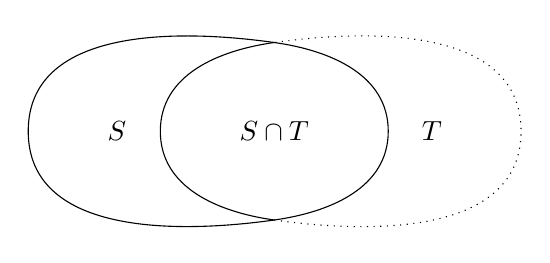
\begin{tikzpicture}[]

\begin{scope}[every node/.style={inner sep=1cm}]
\node(s) at(-2,0) {$S$};
\node(st) at(0,0) {$S \cap T$};
\node(t) at(2,0) {$T$};
\end{scope}

\draw 
(s.west) to[out=90, in=172] 
(st.north) to[out=-8, in=90] 
(st.east) to[out=270, in=8]
(st.south) to[out=188, in=270]
(s.west)
;

\draw[dotted] 
(st.south) to[out=-8, in=270]
(t.east) to[out=90, in=8] 
(st.north) 
;
\draw 
(st.north) to[out=188, in=90] 
(st.west) to[out=270, in=172]
(st.south)
;

\end{tikzpicture}
\end{subfigure}
%
\hfill
%
\begin{subfigure}{.45\linewidth}
\centering
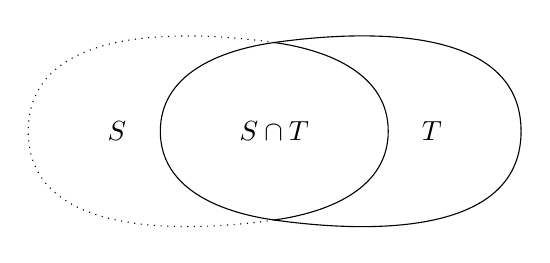
\begin{tikzpicture}[]

\begin{scope}[every node/.style={inner sep=1cm}]
\node(s) at(-2,0) {$S$};
\node(st) at(0,0) {$S \cap T$};
\node(t) at(2,0) {$T$};
\end{scope}

\draw[dotted] 
(st.south) to[out=188, in=270]
(s.west) to[out=90, in=172] 
(st.north)
;
\draw 
(st.north) to[out=-8, in=90] 
(st.east) to[out=270, in=8]
(st.south)
;

\draw 
(t.east) to[out=90, in=8] 
(st.north) to[out=188, in=90] 
(st.west) to[out=270, in=172]
(st.south) to[out=-8, in=270]
(t.east)
;

\end{tikzpicture}
\end{subfigure}
\caption[]{%
Given the two solutions on the left, 
\subref{sub:cup} and \subref{sub:cap}, we
can construct the two solutions on the right side,
\subref{sub:s} and \subref{sub:t}, with equal total weight.
The edges of type 
\inlineedge{e1}, 
\inlineedge{e2}, 
\inlineedge{e3}, 
\inlineedge{e5}, 
\inlineedge{e6}
from the left side are ``naturally'' distributed over the two solutions on the
right side and the edges of type \inlineedge{e4} can be distrebuted between the
two solutions without violating the capacity constraints.
}
\label{fig:sub}
\end{figure}

%%%%%%%%%%%%%%%%%%%%%%%%%%%%%%%%%

\newpage

\section{Tight Analysis}
\label{sec:tight}

We now show that Corollary~\ref{cor:local} is tight.  Consider the
example in Figure~\ref{fig:local search tight}, the example is for the
special case when $k = 11$ and $\cmax = 2$ but this example can be
generalized in a straightforward manner.  One can verify that as the
graph in the example growth, the ratio between the optimal solution
and the local search solution approaches $\frac{3}{4}$.

\begin{figure}[h]
\begin{center}
\scalebox{.85}{\input{fig-local-tight}}
\caption{A tight example for Corollary~\ref{cor:local}. 
The optimal solution is given by the red solid arcs while the local
search solution is given by the green, dashed arcs.  The solution can
be improved by the local search algorithm only if it removes all the
edges.}
\label{fig:local search tight}
\end{center}
\end{figure}

